%\hyperdef{recursive}{data}

\chapter{Recursive Data Types}\label{recursive_data_chapter}

\term{Recursive data types} play a central role in programming, and
induction is really all about them.

Recursive data types are specified by \term{recursive definitions} that
say how to contruct new data elements from previous ones.  Along with each
recursive data type there are recursive definitions of properties or
functions on the data type.  Most importantly, based on a recursive
definition, there is a \term{structural induction} method for proving that
all data of the given type have some property.

This chapter examines a few examples of recursive data types and
recursively defined functions on them:
\begin{itemize}
\item strings of characters,
\item the ``balanced'' strings of brackets,
\item the nonnegative integers, and
\item arithmetic expressions.
%\item two-player zero-sum games with perfect information.
\end{itemize}

%\hyperdef{paren}{string}
\section{Recursive Definitions and Structural Induction}

We'll start off illustrating recursive definitions and proofs using the
example of character strings.  Normally we'd take strings of characters
for granted, we'll treat them as a recursive data type.  Strings make a
nice first example because we're giving recursive definitions of things
that are easy to understand or you already know, so you can focus on how
the definitions work without having to figure out what they are for.

Definition of recursive data types have two parts:
\begin{itemize}
\item \textbf{Base case(s)} specifying that some known mathematical elements are
  in the data type, and

\item \textbf{Constructor case(s)} that specify how to construct new data
  elements from previously contructed element of form base elements.
\end{itemize}

The definition of strings over a given character set, $A$, follows this
pattern:

\begin{definition}\label{recstring_def}
  Let $A$ be a nonempty set called an \term{alphabet}, whose elements are
  referred to as \term{characters}, \term{letters}, or \term{symbols}.
  The recursive data type, $\strings{A}$, of strings over alphabet, $A$,
  are defined as follows:
\begin{itemize}
\item \textbf{base case}: the empty string, $\emptystring$, is in $\strings{A}$.

\item \textbf{constructor case:} If $a \in A$ and $s \in \strings{A}$, then the pair
       $\ang{a,s} \in \strings{A}$.
\end{itemize}
\end{definition}
So $\strings{\set{0,1}}$ are supposed to be the binary strings.

The usual way to treat binary strings is as sequences of 0's and 1's.
For example, we have identified the length-4 binary string 1011 as a
sequence of bits, of a 4-tuple, namely, $(1,0,1,1)$.  But according to
the recursive Definition~\ref{recstring_def}, this string would be
represented by nested pairs, namely
\[
\ang{1,\ang{0,\ang{1,\ang{1,\emptystring}}}}.
\]
These nested pairs are definitely cumbersome, and may also seem
bizarre, but they actually reflect the way lists of characters would
be represented in programming languages like Scheme or Python, where
$\ang{a,s}$ would be correspond to $\text{cons}(a, s)$.

Notice that we haven't said exactly how the empty string is
represented.  It really doesn't matter as long as we can recognize the
empty string and not confuse it with any nonempty string.

Continuing the recursive approach, let's define the length of a string.
\begin{definition}
The length, $\lnth{s}$, of a string, $s$, is defined recursively
based on the definition of $s \in \strings{A}$:

\item \textbf{base case}:  $\lnth{\emptystring} \eqdef\ 0$.

\item \textbf{constructor case}: $\lnth{\ang{a,s}} \eqdef\ 1 + \lnth{s}$.

\end{definition}

This definition of length follows a standard pattern: functions on
recursive data types can be defined recursively using the same cases as
the data type definition.  Namely, to define a function, $f$, on a
recursive data type, define the value of $f$ for the base cases of the
data type definition, and then define the value of $f$ in each constructor
case in terms of the values of $f$ on the component data items.

Let's do another example: the \term{concatenation} $s\cdot t$ of the
strings $s$ and $t$ is the string consisting of the letters of $s$
followed by the letters of $t$.  This is a perfectly clear mathematical
definition of concatenation (except maybe for what to do with the empty
string), and in terms of Scheme/Python lists, $s\cdot t$ would be the list
$\text{append}(s, t)$.  Here's a recursive definition of concatenation.

\begin{definition}\label{concat_def}
The \term{concatenation} $s\cdot t$ of the strings $s,t \in
\strings{A}$ is defined recursively based on the definition of $s \in
\strings{A}$:

\item \textbf{base case}:     % ($s=\emptystring$):
\[
\emptystring \cdot t \eqdef\ t.
\]

\item \textbf{constructor case}: %($s = \ang{a,r}$ for $r \in \strings{A}$):
\[
\ang{a,s} \cdot t \eqdef\ \ang{a, s \cdot t}.
\]
\end{definition}

\term{Structural induction} is a method for proving that all the elements
of a recursively defined data type have some property.  A structural
induction proof has two parts corresponding to the recursive definition:
\begin{itemize}
\item Prove that each base case element has the property.
\item Prove that each constructor case element has the property, when
  the constructor is applied to elements that have the property.
\end{itemize}

For example, we can verify the familiar fact that the length of the
concatenation of two strings is the sum of their lengths using structural
induction:

\begin{theorem}\label{stAl+}
For all $s,t \in \strings{A}$,
\[
\lnth{s\cdot t} = \lnth{s} + \lnth{t}.
\]
\begin{proof}
By structural induction on the definition of $s \in \strings{A}$.   The
induction hypothesis is
\[
P(s) \eqdef\ \forall t \in \strings{A}.\, \lnth{s\cdot t} = \lnth{s} + \lnth{t}.
\]

\textbf{base case} ($s = \emptystring$):
\begin{align*}
\lnth{s \cdot t}
   &= \lnth{\emptystring \cdot t}\\
   & = \lnth{t}
         & \text{(def $\cdot$, base case)}\\
   & = 0 + \lnth{t}\\
   & = \lnth{s} + \lnth{t}
         & \text{(def length, base case)}
\end{align*}
\end{proof}

\textbf{constructor case}: Assume the induction hypothesis, $P(s)$, and
let $r = \ang{a,s} \cdot t$.  We must show that $P(r)$ holds:
\begin{align*}
\lnth{r \cdot t}
    & = \lnth{\ang{a, s} \cdot t}\\
    & = \lnth{\ang{a,s \cdot t}}
        &  \text{(def $\cdot$, constructor case)}\\
    & = 1 + \lnth{s \cdot t}
        &  \text{(def length, constructor case)}\\
    & = 1 +  (\lnth{s} + \lnth{t})
        & \text{since $P(s)$ holds}\\
    & = (1 +  \lnth{s}) + \lnth{t}\\
    & = \lnth{\ang{a,s}} + \lnth{t}
        & \text{(def length, constructor case)}\\
    & = \lnth{r} + \lnth{t}.
\end{align*}
This completes the proof of the constructor case, so by structural
induction we conclude that $P(s)$ holds for all strings $s \in
\strings{A}$.

\end{theorem}

This proof illustrates the general principle:

\textbox{ 
\textboxheader{The Principle of Structural Induction.}

Let $P$ be a predicate on a recursively defined data type $R$.  If
%
\noindent \begin{itemize}
\item $P(b)$ is true for each base case element, $b \in R$, and

\item for all two argument constructors, $\mathbf{c}$,
\[
[P(r)\QAND P(s)] \QIMPLIES P(\mathbf{c}(r, s))
\]
for all $r,s \in R$,\\
and likewise for all constructors taking other numbers of arguments,
\end{itemize}
then
\[
P(r) \text{ is true for all } r \in R.
\]
}

The number, $\cnt{c}{s}$, of occurrences of the character $c \in A$ in
the string $s$ has a simple recursive definition based on the
definition of $s \in \strings{A}$:
\begin{definition}\label{countas_def}

\textbf{base case}: $\cnt{c}{\emptystring} \eqdef\ 0$.

\textbf{constructor case}:
\[
\cnt{c}{\ang{a,s}} \eqdef \begin{cases}
                           \cnt{c}{s}  &\text{ if } a \neq c,\\
                           1 + \cnt{c}{s} &\text{ if } a = c.
                           \end{cases}
\]

\end{definition}

We'll need the following lemma in the next section:
\begin{lemma}\label{countas_lem}
\[
\cnt{c}{s cdot t} = \cnt{c}{s} + \cnt{c}{t}.
\]
\end{lemma}
The proof, which is very similar to the proof of Theorem~\ref{stAl+},
is a simple exercise (see Problem~\ref{PS_count_a_s_lem}).

\begin{problems}
\classproblems
\pinput{CP_string_associativity}
\pinput{CP_string_reversal}
\pinput{CP_F18_functions}
\pinput{CP_recursively_defined_sets}
\pinput{CP_binary_trees}

\homeworkproblems
\pinput{PS_count_a_s_lem}
\pinput{PS_koch_snowflake}
\end{problems}

\section{Strings of Matched Brackets}

Let $\brkts$ be the set of all strings of square brackets.  For example,
the following two strings are in $\brkts$:
\begin{equation}\label{2strings}
\lefbrk\rhtbrk\rhtbrk\lefbrk\lefbrk\lefbrk\lefbrk\lefbrk\rhtbrk\rhtbrk\quad \text{and}\quad \lefbrk\lefbrk\lefbrk\rhtbrk\rhtbrk\lefbrk\rhtbrk\rhtbrk\lefbrk\rhtbrk
\end{equation}

A string, $s \in \brkts$, is called a \term{matched string} if its
brackets ``match up'' in the usual way.  For example, the left hand
string above is not matched because its second right bracket does not
have a matching left bracket.  The string on the right is matched.

We're going to examine several different ways to define and prove
properties of matched strings using recursively defined sets and
functions.  These properties are pretty straightforward, and you might
wonder whether they have any particular relevance in computer scientist.
The honest answer is ``not much relevance, \emph{any more}.''  The reason
for this is one of the great successes of computer science as explained in
the text box below.

\textbox{
\begin{center}
\textbf{\large Expression Parsing}
\end{center}

%Flesh this out and get references

During the early development of computer science in the 1950's and 60's,
creation of effective programming language compilers was a central
concern.  A key aspect in processing a program for compilation was
expression parsing.  The problem was to take in an expression like
\[
x + y * z^2 \div y + 7
\]
and \emph{put in} the brackets that determined how it
should be evaluated ---should it be
\begin{align*}
[[x + y] * z^2 \div y] + 7,\text{ or}, \\
x + [y * z^2 \div [y + 7]], \text{ or},\\
[x + [y * z^2 ]] \div [y + 7],
\end{align*}
or \dots?

The Turing award (the ``Nobel Prize'' of computer science) was ultimately
bestowed on Robert Floyd, for, among other things, being discoverer of a
simple program that would insert the brackets properly.

In the 70's and 80's, this parsing technology was packaged into high-level
compiler-compilers that automatically generated parsers from expression
grammars.  This automation of parsing was so effective that the subject
needed no longer demanded attention.  It largely disappeared from the
computer science curriculum by the 1990's.}

\iffalse
One precise way to determine if a string is matched is to start with 0 and
read the string from left to right, adding 1 to the count for each left
bracket and subtracting 1 from the count for each right bracket.
For example, here are the counts for the two strings above
\[\begin{array}{rrrrrrrrrrrrr}
& \lefbrk & \rhtbrk & \rhtbrk & \lefbrk & \lefbrk & \lefbrk & \lefbrk &
\lefbrk & \rhtbrk & \rhtbrk & \rhtbrk & \rhtbrk\\
0 & 1 & 0 & -1 & 0 & 1 & 2 & 3 & 4 & 3 & 2 & 1 & 0\\
\\
\\
& \lefbrk & \lefbrk & \lefbrk & \rhtbrk & \rhtbrk & \lefbrk & \rhtbrk &
\rhtbrk & \lefbrk & \rhtbrk\\
0 & 1 & 2 & 3 & 2 & 1 & 2 & 1 & 0 & 1 & 0
\end{array}\]
A string has a \term{good count} if its running count never goes
negative and ends with 0.  So the second string above has a good count, but
the first one does not because its count went negative at the third step.
\begin{definition}\label{gc-def}
Let
\[
\GC \eqdef\  \set{ s \in \brkts \suchthat s\ \text{has a good count}}.
\]
\end{definition}
The matched strings can now be characterized precisely as this set of
strings with good counts.
\fi

The matched strings can be nicely characterized as a recursive data type:

\begin{definition}\label{RM-def}
Recursively define the set, $\RM$, of strings as follows:
\begin{itemize}

\item \textbf{Base case:} $\emptystring \in\RM$.

\item \textbf{Constructor case:} If $s,t \in\RM$, then
\[
\lefbrk s\, \rhtbrk t \in \RM.
\]
\end{itemize}

\end{definition}

Here $\lefbrk s\, \rhtbrk t$ refers to the concatenation of
strings which would be written in full as
\[
\lefbrk \cdot (s \cdot (\rhtbrk \cdot t)).
\]
From now on, we'll usually omit the ``$\cdot$'s.'' 

Using this definition, we can see that $\emptystring \in\RM$ by the Base
case, so
\[
\lefbrk\emptystring\rhtbrk\emptystring=\lefbrk\rhtbrk\in\RM
\]
by the Constructor case.  So now,
\begin{align*}
\lefbrk\emptystring\rhtbrk\lefbrk\rhtbrk &= \lefbrk\rhtbrk\lefbrk\rhtbrk \in \RM
    & \text{(letting $s = \emptystring, t = \lefbrk\rhtbrk$)}\\
\lefbrk\lefbrk\rhtbrk\rhtbrk\emptystring & = \lefbrk\lefbrk\rhtbrk\rhtbrk \in \RM
    & \text{(letting $s = \lefbrk\rhtbrk, t = \emptystring$)}\\
&\ \ \lefbrk\lefbrk\rhtbrk\rhtbrk\lefbrk\rhtbrk \in \RM
    & \text{(letting $s = \lefbrk\rhtbrk, t = \lefbrk\rhtbrk$)}
\end{align*}
are also strings in $\RM$ by repeated applications of the Constructor
case.  If you haven't seen this kind of definition before, you should try
continuing this example to verify that
$\lefbrk\lefbrk\lefbrk\rhtbrk\rhtbrk\lefbrk\rhtbrk\rhtbrk\lefbrk\rhtbrk
\in \RM$

\iffalse
Given the way this section is set up, you might guess that $\RM = \GC$,
and you'd be right, but it's not completely obvious.  The proof is worked
out in Problem~\ref{PS_bracket_good_count}.
\fi

With another simple appeal to structural induction we can prove

\begin{lemma*}%label{}
Every string in $\RM$ has an equal number of left and right brackets.

\begin{proof}
The proof is by structural induction with induction hypothesis
\[
P(s) \eqdef\  \cnt{\lefbrk}{s} = \cnt{\rhtbrk}{s}.
\]

\textbf{Base case:} $P(\emptystring)$ holds because
\[
\cnt{\lefbrk}{\emptystring} = 0 = \cnt{\rhtbrk}{\emptystring}
\]
by the base of the definition of count~\ref{countas_def}.

\textbf{constructor case}: By structural induction hypothesis assume
$P(s)$ and $P(t)$ and must show $P(\lefbrk s\,\rhtbrk t)$:
\begin{align*}
\cnt{\lefbrk}{\lefbrk s\,\rhtbrk t}
    & = \cnt{\lefbrk}{\lefbrk} + \cnt{\lefbrk}{s}
        +\cnt{\lefbrk}{\rhtbrk}+ \cnt{\lefbrk}{t}
         & \text{(by Lemma~\ref{countas_lem})}\\
    & = 1 + \cnt{\lefbrk}{s} + 0 + \cnt{\lefbrk}{t}
         & \text{(by def~\ref{countas_def} of $\cnt{\lefbrk}{}$)}\\
    & = 1 + \cnt{\rhtbrk}{s} + 0 + \cnt{\rhtbrk}{t}
         & \text{(by $P(s)$ and $P(t)$)}\\
    & = 0 + \cnt{\rhtbrk}{s} + 1 + \cnt{\rhtbrk}{t}\\
    & = \cnt{\rhtbrk}{\lefbrk} + \cnt{\rhtbrk}{s}
        +\cnt{\rhtbrk}{\rhtbrk}+ \cnt{\rhtbrk}{t}
         & \text{(by def~\ref{countas_def} of $\cnt{\rhtbrk}{}$)}\\
    & = \cnt{\rhtbrk}{\lefbrk s\,\rhtbrk t}
            & \text{(by Lemma~\ref{countas_lem})}
\end{align*}
This completes the proof of the constructor case.  We conclude by
structural induction that $P(s)$ holds for all $s \in\RM$.
\end{proof}
\end{lemma*}


\iffalse

The \term{depth} of a matched string is defined recursively as follows
\begin{definition}
The \emph{depth}, $d(s)$, of a string, $s \in\RM$, is defined
recursively by the rules:
\begin{itemize}
\item $d(\emptystring) \eqdef\  0.$
\item $d(\lefbrk s\,\rhtbrk t)
    \eqdef\ \max \set{d(s) + 1, d(t)}$
\end{itemize}
\end{definition}
\fi

\textbf{Warning:} When a recursive definition of a data type allows
the same element to be constructed in more than one way, the
definition is said to be \emph{ambiguous}.  We were careful to choose
an \emph{un}ambiguous definition of $\RM$ to ensure that functions
defined recursively on its definition would always be well-defined.
Recursively defining a function on an ambiguous of a data type
definition usually will not work.  To illustrate the problem, here's
yet another definition of the matched strings.

\iffalse Recursive definitions of tagged data types, where the tag
uniquely determines the rule used to construct an element, are guaranteed
to be unambiguous.r
\fi

\begin{definition}
\label{M}
Define the set, $\AM \subseteq \brkts$ recursively as follows:
\begin{itemize}

\item \textbf{Base case:} $\emptystring \in \AM$,

\item \textbf{Constructor cases:} if $s,t \in \AM$, then
  the strings $\lefbrk s\, \rhtbrk$ and $st$ are also in $\AM$.
\end{itemize}
\end{definition}

\iffalse
\begin{notesproblem}
Give an easy proof by structural induction that $\AM =\RM$.
\end{notesproblem}
\fi

It's pretty easy to see that the definition of $\AM$ is just another
way to define $\RM$, that is $\AM = \RM$, see
Problem~\ref{PS_M_equal_RM}.  The definition of $\AM$ is arguably
easier to understand, but we didn't use it becaused it's ambiguous,
while the trickier definition of $\RM$ is unambiguous.  Here's why
this matters.  Define the number of operations, $f(s)$, to construct a matched string $s$
recursively on the definition of  $s \in \AM$:
\begin{align*}
  f(\emptystring)        & \eqdef\ 0, \tag{(base case)}\\
  f(\lefbrk s\,\rhtbrk\ ) & \eqdef\ 1+ f(s), \\
  f(st)                  & \eqdef\ 1+ f(s) +f(t).\tag{concat case}
\end{align*}
This definition may seem ok, but it isn't: it implies that
$f(\emptystring)$ is equal to both 0 and 1!  Namely,
\begin{align*}
f(\emptystring) & = 0 & \text{(by (base case))},
\end{align*}
but also,
\begin{align*}
f(\emptystring) & = f(\emptystring \emptystring)\\
                & = 1 + f(\emptystring) + f(\emptystring)
                      &  \text{(by (concat case))},\\
                & = 1 + 0 + 0 = 1
                      & \text{(by (base case))}
\end{align*}

\iffalse

Now suppose $s = \lefbrk\rhtbrk\lefbrk\rhtbrk\lefbrk\rhtbrk\lefbrk\rhtbrk$.


%%FIND SIMPLER EXAMPLE

Let $a$ be the string $\lefbrk\lefbrk\rhtbrk\rhtbrk \in M$ built by two successive
applications of the first $M$ constructor starting with $\emptystring$.  Next
let $b \eqdef aa$ and $c \eqdef bb$, each built by successive applications
of the second $M$ constructor.

Alternatively, we can build $ba$ from the second constructor with $s=b$
and $t=a$, and then get to $c$ using the second constructor with $s=ba$
and $t=a$.

Now by these rules, $f(a) = 2$, and $f(b) = (2+1)(2+1)=9$.  This means
that $f(c) = f(bb)= (9+1)(9+1)=100$.

But also $f(ba) = (9+1)(2+1) = 27$, so that $f(c) = f(ba\,a) = (27 +1)
(2+1) = 84$.

The outcome is that $f(c)$ is defined to be both 100 and 84, which shows
that the rules defining $f$ are inconsistent.

On the other hand, structural induction remains a sound proof method even
for ambiguous recursive definitions, which is why it is easy to prove
that $M=\RM$.
\fi

\begin{problems}

\practiceproblems
\pinput{MQ_ambiguous_recursive-def}

\classproblems
\pinput{CP_erasable_strings}
\pinput{PS_M_equal_RM}
\pinput{PS_bracket_good_count}

\end{problems}


\section{Recursive Functions on Nonnegative Integers}

The nonnegative integers can be understood as a recursive data type.
\begin{definition}\label{0succ}
The set, $\naturals$, is a data type defined recursivly as:
\begin{itemize}
\item $0 \in \naturals$.
\item If $n \in \naturals$, then the \emph{successor}, $n+1$, of $n$ is in
$\naturals$.
\end{itemize}

\end{definition}

This of course makes it clear that ordinary induction is simply the
special case of structural induction on the recursive
Definition~\ref{0succ}.  This also justifies the familiar recursive
definitions of functions on the nonnegative integers.  Here are some
examples.

\begin{description}
\item[The Factorial function.] This function is often written ``$n!$.''
You will see a lot of it later in the term.  Here we'll use the notation
$\text{fac}(n)$:
\begin{itemize}
\item $\text{fac}(0) \eqdef 1$.
\item $\text{fac}(n+1) \eqdef (n+1)\cdot \text{fac}(n)$ for $n \ge 0$.
\end{itemize}

\item[The Fibonacci numbers.]  Fibonacci numbers arose out of an effort 800
  years ago to model population growth.  They have a continuing fan club of
  people captivated by their extraordinary properties.  The $n$th Fibonacci
  number, $\text{fib}$, can be defined recursively by:
\begin{align*}
\text{fib}(0) &\eqdef 0,\\ 
\text{fib}(1) &\eqdef 1,\\ 
\text{fib}(n) &\eqdef \text{fib}(n-1) + \text{fib}(n-2) &\mbox{for $n \geq 2$.} 
\end{align*}
Here the recursive step starts at $n=2$ with base cases for 0 and 1.  This
is needed since the recursion relies on two previous values.

What is $\text{fib}(4)$?  Well, $\text{fib}(2) =
\text{fib}(1)+\text{fib}(0) = 1$, $\text{fib}(3) =
\text{fib}(2)+\text{fib}(1) = 2$, so $\text{fib}(4) = 3$.  The sequence
starts out $0, 1, 1, 2, 3, 5, 8, 13, 21,\dots$.


\item[Sum-notation.]  Let ``$S(n)$'' abbreviate the expression
``$\sum_{i=1}^n f(i)$.''  We can recursively define $S(n)$ with the rules
  \begin{itemize}
  \item $S(0) \eqdef 0$.
  \item $S(n+1) \eqdef  f(n+1) + S(n)$ for $n\geq 0$.
  \end{itemize}

\begin{staffnotes}

\item[Simultaneous recursive definitions:]
  You can define several things at the same time, in terms of each
  other.  For example, we may define two functions $f$ and $g$ from
  $\naturals$ to $\naturals$, recursively, by:
  \begin{itemize}
  \item
    $f(0) \eqdef 1$,
  \item
    $g(0) \eqdef 1$,
  \item
    $f(n+1) \eqdef f(n) + g(n)$, for $n \geq 0$,
  \item
    $g(n+1) \eqdef f(n) \times g(n)$, for $n \geq 0$.
  \end{itemize}

\end{staffnotes}

\end{description}

\begin{staffnotes}

\subsection{Induction on Fibonacci Numbers}

We can use the recursive definition of a function to establish its
properties by structural induction.

As an illustration, we'll prove a cute identity involving Fibonacci
numbers.  Fibonacci numbers provide lots of fun for mathematicians because
they satisfy many such identities.
\begin{proposition}
  $\forall n \geq 0 (\Sigma_{i=0}^n F_i^2 = F_n F_{n+1})$.
\end{proposition}

Example: $n = 4$:
\[
0^2 + 1^2 + 1^2 + 2^2 + 3^2 = 15 = 3 \cdot 5.
\]
Let's try a proof by (standard, not strong) induction.  The theorem
statement suggests trying it with $P(n)$ defined as:
\[
\sum_{i=0}^n F_i^2 = F_n F_{n+1}.
\]

\textbf{Base case} ($n=0$). 
$\Sigma_{i=0}^0 F_i^2 \eqdef (F_0)^2 = 0 = F_0 F_1$ because
$F_0 \eqdef 0$.

\textbf{Inductive step} ($n\geq 0$).  Now we stare at the gap between
$P(n)$ and $P(n+1)$.  $P(n+1)$ is given by a summation that's obtained
from that for $P(n)$ by adding one term; this suggests that, once again,
we subtract.  The difference is just the term $F_{n+1}^2$.  Now, we are
assuming that the original $P(n)$ summation totals $F_n F_{n+1}$ and want
to show that the new $P(n+1)$ summation totals $F_{n+1} F_{n+2}$.  So we
would {\em like\/} the difference to be
\[
F_{n+1} F_{n+2} - F_n F_{n+1}.
\]

So, the actual difference is $F_{n+1}^2$ and the difference we want is
$F_{n+1} F_{n+2} - F_n F_{n+1}$.  Are these the same?  We want to check
that:
\[
F_{n+1}^2 = F_{n+1} F_{n+2} - F_n F_{n+1}.
\]
But this is true, because it is really the Fibonacci definition in
disguise: to see this, divide by $F_{n+1}$.

\end{staffnotes}

\subsection{Ill-formed Function Definitions}

Besides ambiguous definitions, there are some other
\hyperdef{ill}{formed}{blunders} to watch out for when defining
functions recursively.  Below are some function specifications that
resemble good definitions of functions on the nonnegative integers,
but they aren't.

\begin{eqnarray}\label{f1}
f_1(n)\eqdef 2+f_1(n-1).
\end{eqnarray}
This ``definition'' has no base case.  If some function, $f_1$,
satisfied~(\ref{f1}), so would a function obtained by adding a constant to
the value of $f_1$.  So equation~(\ref{f1}) does not uniquely define
an $f_1$.

\begin{eqnarray}\label{f2}
f_2(n) \eqdef
\begin{cases}
 0, & \text{if $n=0$},\\
 f_2(n+1) &  \text{otherwise}.
\end{cases}
\end{eqnarray}
This ``definition'' has a base case, but still doesn't uniquely determine
$f_2$.  Any function that is 0 at 0 and constant everywhere else would
satisfy the specification, so~\eqref{f2} also does not uniquely define
anything.

In a typical programming language, evaluation of $f_2(1)$ would begin with
a recursive call of $f_2(2)$, which would lead to a recursive call of
$f_2(3)$, \dots with recursive calls continuing without end.  This
``operational'' approach interprets~\eqref{f2} as defining a
\emph{partial} function, $f_2$, that is undefined everywhere but 0.

\begin{eqnarray}\label{f3}
f_3(n) \eqdef \begin{cases}
  0, &  \text{if $n$ is divisible by 2,}\\
  1, &  \text{if $n$ is divisible by 3,}\\
  2, & \text{otherwise.}
 \end{cases}
\end{eqnarray}
This ``definition'' is inconsistent: it requires $f_3(6) = 0$ and $f_3(6)
=1$, so~(\ref{f3}) doesn't define anything.

%\subsubsection{A Mysterious Function}
Mathematicians have been wondering about this function specification for a
while:
\begin{eqnarray}\label{f5}
f_4(n) \eqdef\begin{cases}
 1, & \text{if $n\le 1$},\\
 f_4(n/2) &  \text{if $n>1$ is even},\\
 f_4(3n+1)& \text{if $n>1$ is odd}.
\end{cases}
\end{eqnarray}
For example, $f_4(3)=1$ because
\[
f_4(3)\eqdef f_4(10)\eqdef f_4(5)\eqdef f_4(16)\eqdef f_4(8)\eqdef
f_4(4)\eqdef f_4(2)\eqdef f_4(1)\eqdef 1.
\]
The constant function equal to 1 will satisfy~\eqref{f5} (why?), but it's not
known if another function does too.  The problem is that the third case
specifies $f_4(n)$ in terms of $f_4$ at arguments larger than $n$, and so
cannot be justified by induction on $\naturals$.  It's known that any
$f_4$ satisfying~\eqref{f5} equals 1 for all $n$ up to over a billion.

\iffalse
\textbf{Quick exercise:} Why does the constant function 1
satisfy~\eqref{f5}?
\fi


\section{Arithmetic Expressions}
Expression evaluation is a key feature of programming languages, and
recognition of expressions as a recursive data type is a key to
understanding how they can be processed.

To illustrate this approach we'll work with a toy example: arithmetic
expressions like $3x^2 + 2x + 1$ involving only one variable, ``$x$.''
We'll refer to the data type of such expressions as $\aexp$.  Here is its
definition:

\begin{definition}

\begin{itemize}
\item \textbf{Base cases:}

\begin{enumerate}

\item The variable, $x$, is in $\aexp$.

\item The arabic numeral, $\mtt{k}$, for any nonnegative integer, $k$, is
  in $\aexp$.

\end{enumerate}

\item \textbf{Constructor cases:} If $e,f \in \aexp$, then
\begin{enumerate}
\setcounter{enumi}{2}

\item $\lefbrk e \sumsym f \rhtbrk \in \aexp$.  The expression $\lefbrk e \sumsym
  f \rhtbrk$ is called a \emph{sum}.  The \aexp's $e$ and $f$ are called the
  \emph{components} of the sum; they're also called the \emph{summands}.

\item $\lefbrk e \prodsym f\rhtbrk \in \aexp$.  The expression $\lefbrk e \prodsym f\rhtbrk$ is called a
  \emph{product}.  The \aexp's $e$ and $f$ are called the
  \emph{components} of the product; they're also called the
  \emph{multiplier} and \emph{multiplicand}.

\item $\minussym\lefbrk e\rhtbrk \in \aexp$.  The expression $\minussym\lefbrk e\rhtbrk$ is called a
  \emph{negative}.
\end{enumerate}
\end{itemize}
\end{definition}

Notice that \aexp's are fully parenthesized, and exponents aren't allowed.
So the $\aexp$ version of the polynomial expression $3x^2 + 2x + 1$ would
officially be written as
\begin{equation}\label{fullparens}
\lefbrk \lefbrk \mtt{3} \prodsym \lefbrk x \prodsym x\rhtbrk\rhtbrk \sumsym \lefbrk \lefbrk \mtt{2} \prodsym x\rhtbrk \sumsym \mtt{1}\rhtbrk\rhtbrk.
\end{equation}
These brackets and $\ast$'s clutter up examples, so we'll often use
simpler expressions like ``$3x^2 + 2x + 1$'' instead
of~\eqref{fullparens}.  But it's important to recognize that $3x^2 +
2x + 1$ is not an \aexp; it's an \emph{abbreviation} for an $\aexp$.

\iffalse

being represented as
a tagged datum.  To start, we might represent 0 as a length one sequence
consisting of the tag \texttt{zero}:
\begin{definition}
The nonnegative integers can be defined recursively as follows:

\begin{definition}\label{tagn}
\begin{itemize}
\item \textbf{Base case}  $\ang{\texttt{zero}}\in \naturals$.
\item \textbf{Constructor case} if $n \in \naturals$, then
      $\ang{\texttt{successor},n}\in \naturals$.
\end{itemize}

\end{definition}
\fi

\subsection{Evaluation and Substitution with Aexp's}

\subsubsection{Evaluating Aexp's}

Since the only variable in an \aexp\ is $x$, the value of an \aexp\ is
determined by the value of $x$.  For example, if the value of $x$ is 3,
then the value of $3x^2 + 2x + 1$ is obviously 34.  In general, given any
$\aexp$, $e$, and an integer value, $n$, for the variable, $x$, we can
evaluate $e$ to finds its value, $\meval(e,n)$.  It's easy, and useful, to
specify this evaluation process with a recursive definition.

\begin{definition}\label{meval-def}
  The \term{evaluation function}, $\meval: \aexp \times \integers \to
  \integers$, is defined recursively on expressions, $e \in \aexp$, as
  follows.  Let $n$ be any integer.

\begin{itemize}
\item \textbf{Base cases:}

\begin{enumerate}

\item\label{eval-var} Case[$e$ is $x$]
\[
\meval(x, n) \eqdef n.
\]
(The value of the variable, $x$, is given to be $n$.)

\item\label{eval-const} Case[$e$ is $k$]
\[
\meval(\mtt{k}, n) \eqdef k.
\]
(The value of the numeral $\mtt{k}$ is the integer $k$, no matter what
value $x$ has.)

\end{enumerate}

\item \textbf{Constructor cases:}

\begin{enumerate}
\setcounter{enumi}{2}

\item\label{eval-sum} Case[$e$ is $\lefbrk e_1 \sumsym e_2 \rhtbrk$]
\[
\meval(\lefbrk e_1 \sumsym e_2 \rhtbrk,n) \eqdef
  \meval(e_1,n)+\meval(e_2,n).
\]

\item\label{eval-prod} Case[$e$ is $\lefbrk e_1 \prodsym e_2 \rhtbrk$]
\[
\meval(\lefbrk e_1 \prodsym e_2 \rhtbrk,n) \eqdef \meval(e_1,n) \cdot \meval(e_2,n).
\]

\item\label{eval-minus} Case[$e$ is $\minussym\lefbrk e_1 \rhtbrk$]
\[
\meval(\minussym\lefbrk e_1 \rhtbrk,n) \eqdef - \meval(e_1,n).
\]
\end{enumerate}

\end{itemize}

\end{definition}

For example, here's how the recursive definition of $\meval$ would arrive at
the value of $3+x^2$ when $x$ is 2:
\begin{align*}
\meval(\lefbrk \mtt{3} \sumsym \lefbrk x \prodsym x\rhtbrk \rhtbrk,2)
 & = \meval(\mtt{3},2) + \meval(\lefbrk x \prodsym x \rhtbrk,2)
                  & \text{(by~Def~\ref{meval-def}.\ref{eval-sum})}\\
 & = 3 + \meval(\lefbrk x \prodsym x \rhtbrk,2) & \text{(by~Def~\ref{meval-def}.\ref{eval-const})}\\
 & = 3 + (\meval(x,2) \cdot \meval(x,2)) & \text{(by~Def~\ref{meval-def}.\ref{eval-prod})}\\
 & = 3 + (2 \cdot 2) & \text{(by~Def~\ref{meval-def}.\ref{eval-var})}\\
 & = 3 + 4 = 7.
\end{align*}

\subsubsection{Substituting into Aexp's}
Substituting expressions for variables is a standard, important
operation.  For example the result of substituting the expression $3x$
for $x$ in the expression $\lefbrk x\lefbrk x-1 \rhtbrk \rhtbrk$ would
be $\lefbrk 3x\lefbrk 3x-1 \rhtbrk \rhtbrk$.  We'll use the general
notation $\msubst{f}{e}$ for the result of substituting an $\aexp$,
$f$, for each of the $x$'s in an $\aexp$, $e$.  So as we just explained,
\[
\msubst{3x}{x\lefbrk x-1\rhtbrk} = 3x\lefbrk 3x-1\rhtbrk.
\]

This substitution function has a simple recursive definition:

\begin{definition}\label{subst-def}
  The \term{substitution function} from $\aexp \times \aexp$ to \aexp\ is
  defined recursively on expressions, $e \in \aexp$, as follows.  Let $f$
  be any $\aexp$.

\begin{itemize}
\item \textbf{Base cases:}

\begin{enumerate}

\item\label{subst-var} Case[$e$ is $x$]
\[
\msubst{f}{x} \eqdef f.
\]
(The result of substituting $f$ for the variable, $x$, is just $f$.)

\item\label{subst-const} Case[$e$ is $\mtt{k}$]
\[
\msubst{f}{\mtt{k}} \eqdef \mtt{k}.
\]
(The numeral, $\mtt{k}$, has no $x$'s in it to substitute for.)

\end{enumerate}

\item \textbf{Constructor cases:}

\begin{enumerate}
\setcounter{enumi}{2}
\item\label{subst-sum} Case[$e$ is $(e_1 \sumsym e_2)$]
\[
\msubst{f}{\lefbrk e_1 \sumsym e_2\rhtbrk} \eqdef  \lefbrk \msubst{f}{e_1} \sumsym
\msubst{f}{e_2}\rhtbrk.
\]

\item\label{subst-prod} Case[$e$ is $(e_1 \prodsym e_2)$]
\[
\msubst{f}{\lefbrk e_1 \prodsym e_2\rhtbrk}) \eqdef  \lefbrk \msubst{f}{e_1} \prodsym
\msubst{f}{e_2}\rhtbrk.
\]

\item\label{subst-minus} Case[$e$ is $\minussym\lefbrk e_1\rhtbrk$]
\[
\msubst{f}{\minussym\lefbrk e_1\rhtbrk} \eqdef \minussym \lefbrk \msubst{f}{e_1}\rhtbrk.
\]

\end{enumerate}
\end{itemize}
\end{definition}

Here's how the recursive definition of the substitution function would find
the result of substituting $3x$ for $x$ in the $x(x-1)$:
\begin{align*}
\lefteqn{\msubst{3x}{\lefbrk x\lefbrk x-1\rhtbrk\rhtbrk}}\\
 & =
\msubst{3x}{\lefbrk x \prodsym \lefbrk x \sumsym \minussym\lefbrk 1 \rhtbrk \rhtbrk \rhtbrk} & \text{(unabbreviating)}\\
 & =\lefbrk \msubst{3x}{x} \prodsym \msubst{3x}{\lefbrk x \sumsym \minussym
\lefbrk 1 \lefbrk rhtbrk \rhtbrk}
         & \text{(by~Def~\ref{subst-def}~\ref{subst-prod})}\\
 & = \lefbrk 3x \prodsym \msubst{3x}{\lefbrk x \sumsym \minussym\lefbrk 1 \rhtbrk \rhtbrk} \rhtbrk
         & \text{(by~Def~\ref{subst-def}~\ref{subst-var})}\\
 & = (3x \prodsym \lefbrk \msubst{3x}{x} \sumsym \msubst{3x}{\minussym\lefbrk 1 \rhtbrk} \rhtbrk \rhtbrk
         & \text{(by~Def~\ref{subst-def}~\ref{subst-sum})}\\
 & = \lefbrk 3x \prodsym \lefbrk 3x \sumsym \minussym \lefbrk \msubst{3x}{1} \rhtbrk \rhtbrk \rhtbrk
         & \text{(by~Def~\ref{subst-def}~\ref{subst-var} \&~\ref{subst-minus})}\\
 & = \lefbrk 3x \prodsym \lefbrk 3x \sumsym \minussym \lefbrk 1\rhtbrk \rhtbrk
         & \text{(by~Def~\ref{subst-def}~\ref{subst-const})}\\
 & = 3x\lefbrk 3x-1 \rhtbrk & \text{(abbreviation)}
\end{align*}

Now suppose we have to find the value of $\msubst{3x}{\lefbrk x\lefbrk
  x-1 \rhtbrk \rhtbrk}$ when $x = 2$.  There are two approaches.

First, we could actually do the substitution above to get $3x(3x-1)$,
and then we could evaluate $3x\lefbrk 3x-1 \rhtbrk$ when $x =2$, that
is, we could recursively calculate $\meval(3x\lefbrk 3x-1 \rhtbrk,2)$
to get the final value 30.  In programming jargon, this would be
called evaluation using the \emph{Substitution Model}.  Tracing
through the steps in the evaluation, it turns out that the Substitution
Model requires two substitutions for occurrences of $x$ and 5 integer
operations: 3 integer multiplications, 1 integer addition, and 1
integer negative operation.  In this Substitution Model, the
multiplication $3 \cdot 2$ was performed twice to get the value of 6
for each of the two occurrences of $3x$.

The other approach is called evaluation using the \emph{Environment
  Model}.  Namely, we evaluate $3x$ when $x = 2$ using just 1
multiplication to get the value 6.  Then we evaluate $x\lefbrk x-1
\rhtbrk$ when $x$ has this value 6 to arrive at the value $6\cdot
5=30$.  So the Environment Model requires 2 variable lookups and only
4 integer operations: 1 multiplication to find the value of $3x$,
another multiplication to find the value $6 \cdot 5$, along with 1
integer addition and 1 integer negative operation.

So the Environment Model approach of calculating
\[
\meval(x\lefbrk x-1 \rhtbrk, \meval(3x,2))
\]
instead of the Substitution Model approach of calculating
\[
\meval(\msubst{3x}{x\lefbrk x-1 \rhtbrk},2)
\]
is faster.  But how do we know that these final values reached by these
two approaches always agree?  We can prove this easily by structural
induction on the definitions of the two approaches.  More precisely, what
we want to prove is

\begin{theorem}\label{environments}
For all expressions $e,f \in \aexp$ and $n \in \integers$,
\begin{equation}\label{eval-subst}
\meval(\msubst{f}{e},n) = \meval(e, \meval(f,n)).
\end{equation}
\end{theorem}

\begin{proof}
The proof is by structural induction on $e$.\footnote{This is an
  example of why it's useful to notify the reader what the induction
  variable is---in this case it isn't $n$.}

\textbf{Base cases:}
\begin{itemize}

\item Case[$e$ is $x$]

  The left hand side of equation~\eqref{eval-subst} equals $\meval(f,n)$
  by this base case in Definition~\ref{subst-def} of the substitution
  function, and the right hand side also equals $\meval(f,n)$ by this base
  case in Definition~\ref{meval-def} of $\meval$.


\item Case[$e$ is $\mtt{k}$].

  The left hand side of equation~\eqref{eval-subst} equals $\mtt{k}$ by
  this base case in Definitions~\ref{subst-def} and~\ref{meval-def} of
  the substitution and evaluation functions.  Likewise, the right hand
  side equals $\mtt{k}$ by two applications of this base case in the
  Definition~\ref{meval-def} of $\meval$.

\end{itemize}

\textbf{Constructor cases}:
\begin{itemize}

\item Case[$e$ is $\lefbrk e_1 \sumsym e_2 \rhtbrk$]

  By the structural induction hypothesis~\eqref{eval-subst}, we may assume
  that for all $f \in \aexp$ and $n \in \integers$,

\begin{equation}\label{ln4.hyp}
\meval(\msubst{f}{e_i},n)  =  \meval(e_i, \meval(f,n))
\end{equation}
for $i= 1,2$.  We wish to prove that

\begin{equation}\label{s+}
\meval(\msubst{f}{\lefbrk e_1\sumsym e_2 \rhtbrk},n)  =  \meval(\lefbrk e_1 \sumsym e_2 \rhtbrk, \meval(f,n))
\end{equation}

But the left hand side of~\eqref{s+} equals
\[
\meval(\, \lefbrk \msubst{f}{e_1} \sumsym \msubst{f}{e_2} \rhtbrk,\ n)
\]
by Definition~\ref{subst-def}.\ref{subst-sum} of substitution into a sum
expression.  But this equals
\[
\meval(\msubst{f}{e_1},n) + \meval(\msubst{f}{e_2},n)
\]
by Definition~\ref{meval-def}.\ref{eval-sum} of $\meval$ for a sum expression.  By
induction hypothesis~\eqref{ln4.hyp}, this in turn equals
\[
\meval(e_1,\meval(f,n)) + \meval(e_2,\meval(f,n)).
\]
Finally, this last expression equals the right hand side of~(\ref{s+}) by
Definition~\ref{meval-def}.\ref{eval-sum} of $\meval$ for a sum
expression.  This proves~(\ref{s+}) in this case.

\item $e$ is $\lefbrk e_1 \prodsym e_2 \rhtbrk$.  Similar.

\item $e$ is $-\lefbrk e_1 \rhtbrk$.  Even easier.

\end{itemize}

This covers all the constructor cases, and so completes the proof by
structural induction.

\end{proof}


\begin{staffnotes}

\begin{example*}
\begin{definition}\label{E}
Define a set, $E$, recursively as follows:
\begin{itemize}
\item \textbf{Base case:} $0 \in E$,\label{0E}
\item \textbf{Constructor cases:} if $n \in E$, then
\begin{enumerate}
\item $n+2 \in E$, when $n\geq 0$;\label{+2E}
\item $-n \in E$, when $n > 0$.\label{-E}
\end{enumerate}
\end{itemize}

\end{definition}
\end{example*}

Using this definition, we can see that $0 \in E$ by the Base case, so $0 +
2 = 2 \in E$ by Constructor case~\ref{+2E}., and so $2+2 =4 \in E$, $4+2 =
6 \in E$, \dots, and in fact any nonnegative even number is in $E$ by
successive application of case~\ref{+2E}.  Also, by case~\ref{-E}.,
$-2,-4,-6,\dots \in E$.  So clearly all the even integers are in $E$.

Is anything else in $E$?  The definition doesn't say so explicitly, but an
implicit condition on a recursive definition is that the only way things
get into $E$ is as a consequence of the Base and Constructor cases.  In
other words, $E$ will be exactly the set of even integers.

A very simple application of structural induction proves that the set $E$
given by Definition~\ref{E} is exactly the set of even numbers.  We already
explained why all the even numbers are in $E$.  So what's left is to show
that:

\begin{lemma*}
Every number in the set $E$ in Definition~\ref{E} is even.
\begin{proof}
The proof is by structural induction on $n \in E$.  The induction
hypothesis is 
\[
Q(n) \eqdef \text{$n$ is even}.
\]

\textbf{Base case}: $Q(0)$ holds since 0 is even.

\textbf{Constructor cases}: assuming $n \in E$ and $Q(n)$ holds, prove
that
\begin{itemize}

\item $Q(n+2)$ holds.  This is immediate, since adding 2 to an even number
  gives an even number.

\item $Q(-n)$ holds.  This is also immediate, since $n$ is even iff $-n$ is
even.

\end{itemize}

This completes the proof of the Constructor cases, and we conclude by
structural induction at $Q(n)$ holds for all $n \in E$.
\end{proof}

\end{lemma*}


defining the set, $E$, of even numbers as in Definitions~\ref{E}, but
without the conditions~\ref{+2E}.\ and~\ref{-E}.\ that restrict application of
the rules.  Namely,

\begin{definition}\label{Eamb}
Define a set, $E'$, recursively as follows:
\begin{itemize}
\item \textbf{Base case:} $0 \in E'$,\label{0Eamb}
\item \textbf{Constructor cases:} if $n \in E'$, then
\begin{enumerate}
\item $n+2 \in E'$, \label{+2Eamb}
\item $-n \in E'$.\label{-Eamb}
\end{enumerate}
\end{itemize}
\end{definition}

Now Definition~\ref{Eamb} is perfectly legitimate, and we could us it to
prove by structural induction that $E'$ also is the set of even integers,
that is, $E'= E$.  But Definition~\ref{Eamb} is ambiguous.  For example,
$0\in E'$ by the base case, but also $0=-0 \in E'$ by applying constructor
case~\ref{-Eamb} to the base case.  This begins to matter when we try to
define a function, $s$, from $E'$ to nonnegative integers based on
Definition~\ref{Eamb}:
\begin{align*}
  s(0) & \eqdef 1,\\
s(n+2) & \eqdef 1+ s(n),\\
 s(-n) & \eqdef 1+ s(n).
\end{align*}
So $s(0) \eqdef 1$ by the base case of this definition, and also $s(0)=
s(-0) \eqdef 1+s(0) = 1 + 1 = 2$ by the second constructor case, which
shows that these rules are inconsistent.

On the other hand, using the unambiguous Definition~\ref{E} of $E$,
essentially the same definition of $S$ works just fine.  Namely, define
\begin{align*}
  s(0) & \eqdef 1,\\
  s(n+2) & \eqdef 1+ s(n), & \text{ for } n \geq 0\\
  s(-n) & \eqdef 1+ s(n) & \text{ for } n > 0.
\end{align*}
Now $s(n)$ is unambiguously defined, and in fact is precisely the (unique)
number of steps required to construct $n \in E$ according to the
unambiguous Definition~\ref{E} of $E$.

\end{staffnotes}


\iffalse

%% Games as a Recursive Data Type %%%%%%%%%%%%%%%%%%%%%%%%%%%%%%%%%%%%%%%%%%%%%
\section{Games as a Recursive Data Type}

Chess, Checkers, Go, and Tic-Tac-Toe are examples of \emph{two-person
  terminating games of perfect information}, ---$\tg$'s for short.  These
are games in which two players alternate moves that depend only on the
visible board position or state of the game.  ``Perfect information''
means that the players know the complete state of the game at each move.
(Most card games are \emph{not} games of perfect information because
neither player can see the other's hand.)  ``Terminating'' means that play
cannot go on forever ---it must end after a finite number of
moves.\footnote{Since board positions can repeat in chess and checkers,
  termination is enforced by rules that prevent any position from being
  repeated more than a fixed number of times.  So the ``state'' of these
  games is the board position \emph{plus} a record of how many times
  positions have been reached.}

We will define $\tg$'s \iffalse in a straightforward way tagged\fi as a 
recursive data type.  To see how this will work, let's use the game of
Tic-Tac-Toe as an example.

\subsection{Tic-Tac-Toe}

Tic-Tac-Toe is a game for young children.  There are two players who
alternately write the letters ``X'' and ``O'' in the empty boxes of a $3
\times 3$ grid.  Three copies of the same letter filling a row, column, or
diagonal of the grid is called a \emph{tic-tac-toe}, and the first player
who gets a tic-tac-toe of their letter wins the game.

\begin{staffnotes}
Children generally don't take long to figure out an optimal strategy
for playing the game.
\end{staffnotes}

We're now going give a precise mathematical definition of the Tic-Tac-Toe
\term{game tree} as a recursive data type.  \iffalse and carefully defining
the allowed moves\fi
\begin{staffnotes}
Children of course have no need for such a definition, and it would be
too complicated for them anyway.  But if we had to write a Tic-Tac-Toe
playing \emph{computer program}, we'd need this kind of picky
precision.
\end{staffnotes}

Here's the idea behind the definition: at any point in the game, the
``board position'' is the pattern of X's and O's on the $3 \times 3$
grid.  From any such Tic-Tac-Toe pattern, there are a number of next
patterns that might result from a move.  For example, from the initial
empty grid, there are nine possible next patterns, each with a single
X in some grid cell and the other eight cells empty.  From any of
these patterns, there are eight possible next patterns gotten by
placing an O in an empty cell.  These move possibilities are given by
the
\hyperdef{game}{tree}{game tree} for Tic-Tac-Toe indicated in
Figure~\ref{fig:Tic-Tac-Toe}.

\begin{figure}
%\graphic{topgame}
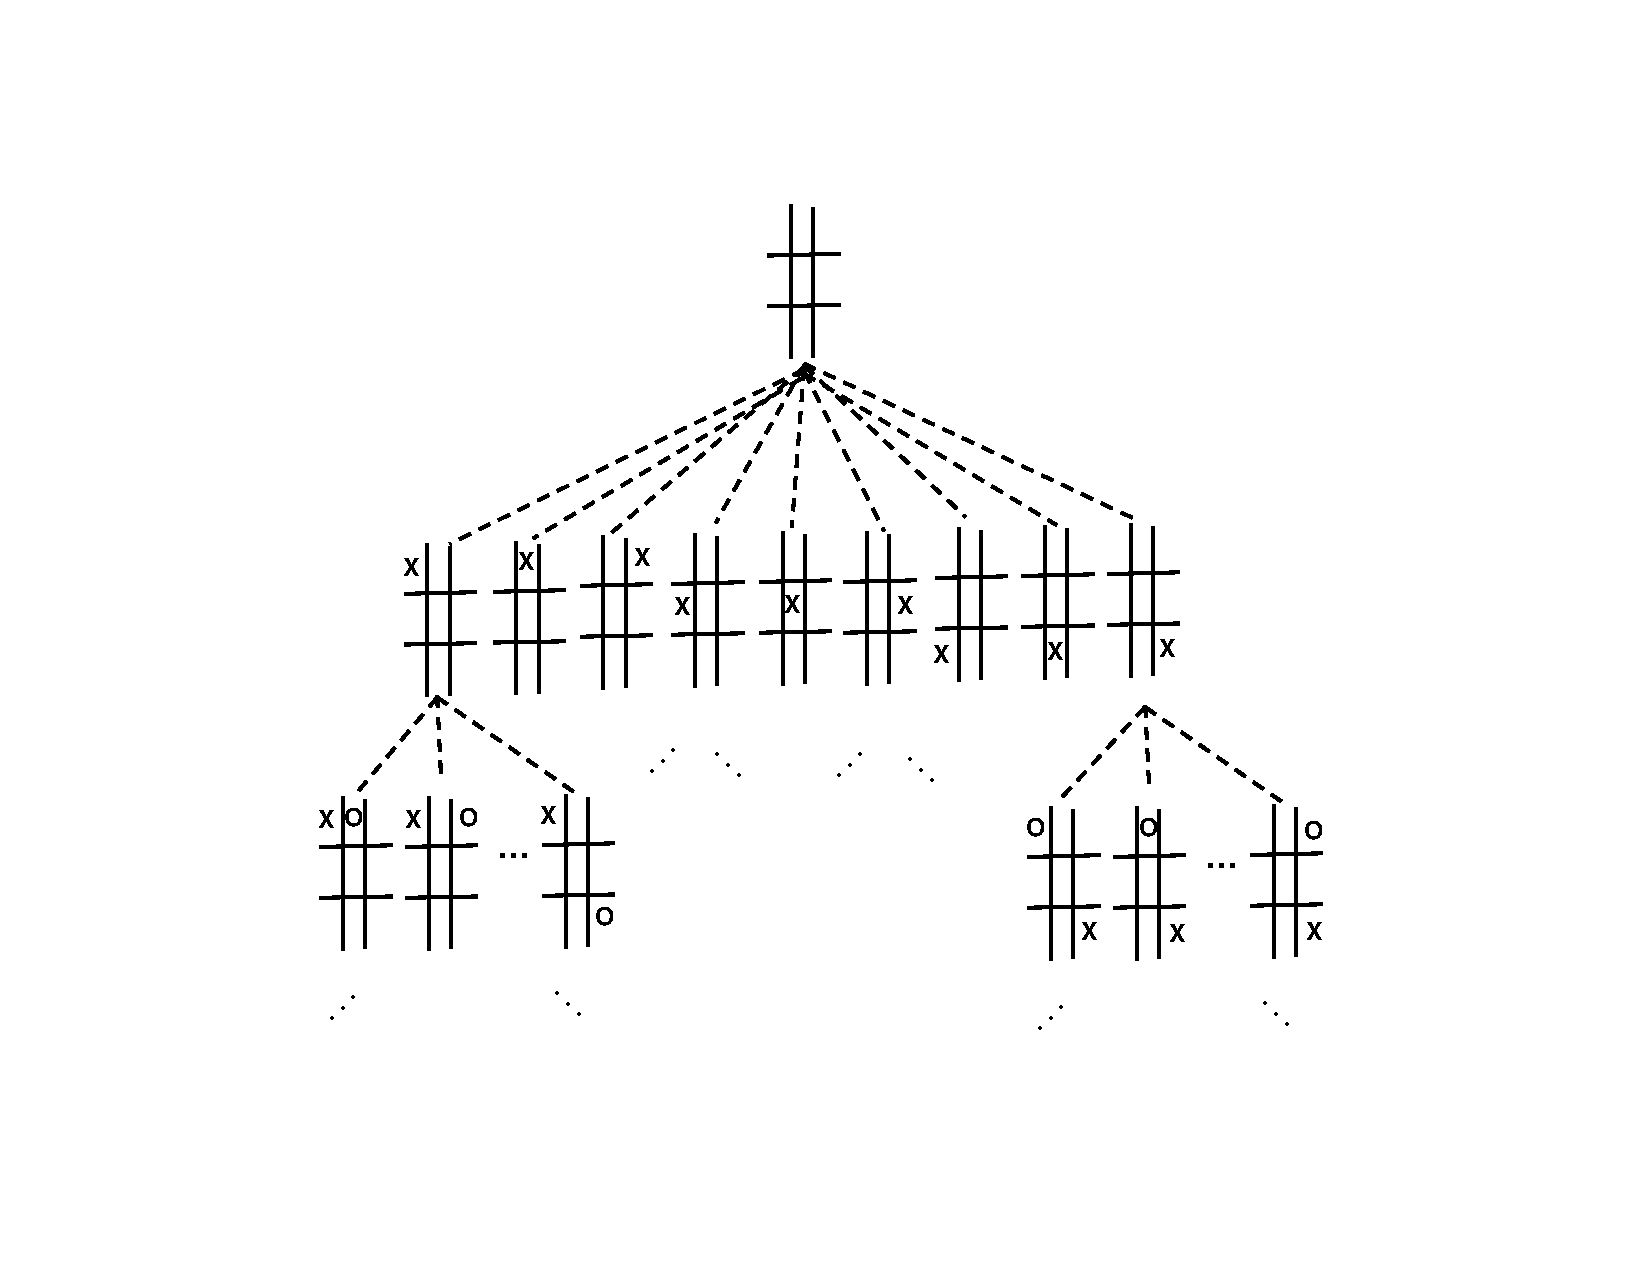
\includegraphics[width=6.5in]{topgame}
\caption{The Top of the Game Tree for Tic-Tac-Toe.}
\label{fig:Tic-Tac-Toe}
\end{figure}


\iffalse
\[\begin{array}{c|c|c}
\hspace{.1in} & \hspace{.1in} & \hspace{.1in}\\
\hline  & &\\
\hline  & &
\end{array}\]

\textbf{FIGURE NEEDED}
\fi

\begin{definition}

A Tic-Tac-Toe \emph{pattern} is a $3 \times 3$ grid each of whose 9 cells
contains either the single letter, X, the single letter, O, or is
empty.
\begin{staffnotes}

Moreover, there must be either
\begin{itemize}

\item one more X than O's, with at most two tic-tac-toes of X's, and no
tic-tac-toe of O's, or

\item an equal number of X's and O's, with at most one tic-tac-toes of
O's, and no tic-tac-toe of X's.
\end{itemize}

\end{staffnotes}

A pattern, $Q$, is a \emph{possible next pattern after} $P$, providing $P$
has no tic-tac-toes and
\begin{itemize}

\item if $P$ has an equal number of X's and O's, and $Q$ is the same as
$P$ except that a cell that was empty in $P$ has an X in $Q$, or

\item if $P$ has one more X than O's, and $Q$ is the same as $P$ except
that a cell that was empty in $P$ has an O in $Q$.
\end{itemize}

If $P$ is a Tic-Tac-Toe pattern, and $P$ has no next patterns, then the
\emph{terminated Tic-Tac-Toe game trees} at $P$ are

\begin{itemize}

\item 
$\ang{P, \ang{\texttt{win}}}$,
if $P$ has a tic-tac-toe of X's.


\item 
$\ang{P, \ang{\texttt{lose}}}$, if $P$ has a tic-tac-toe of O's.


\item $\ang{P, \ang{\texttt{tie}}}$, otherwise.

\end{itemize}

\iffalse
If $Q$ is a possible move from $P$, then the game tree starting at $Q$ is
called a \emph{  Notice
that $\mathcal{G}_P = \emptyset$ iff $P$ is terminated.}
\fi

The \emph{Tic-Tac-Toe game trees starting at $P$} are defined recursively:

\textbf{Base Case}:
A terminated Tic-Tac-Toe game tree at $P$ is a Tic-Tac-Toe game tree
starting at $P$.

\textbf{Constructor case}: If $P$ is a non-terminated Tic-Tac-Toe pattern,
then the Tic-Tac-Toe game tree starting at $P$ consists of $P$ and the set
of all game trees starting at possible next patterns after $P$.
\end{definition}

For example, if
\begin{align*}
P_0 & =  \begin{array}{c|c|c}
                O & X & O\\
         \hline X & O & X\\
         \hline X & &
        \end{array}\\
Q_1 & = \begin{array}{c|c|c}
                O & X & O\\
         \hline X & O & X\\
         \hline X &  & O
        \end{array}\\
Q_2 & = \begin{array}{c|c|c}
                O & X & O\\
         \hline X & O & X\\
         \hline X & O & 
        \end{array}\\
R & = \begin{array}{c|c|c}
                O & X & O\\
         \hline X & O & X\\
         \hline X & O & X
        \end{array}
\end{align*}
the game tree starting at $P_0$ is pictured in Figure~\ref{fig:endgame}.

\begin{staffnotes}

Then,
\begin{equation}\label{endgame}
\ang{P, \set{\ang{Q_1, \ang{\texttt{lose}}},
             \ang{Q_2, \set{\ang{R,\ang{\texttt{tie}}}}}}}
\end{equation}
is the tagged recursive datum that corresponds to a Tic-Tac-Toe ``end
game'' that starts with $P$.  This game is easier to understand by looking
at its game tree in Figure~\ref{fig:endgame}.  Notice that the game tree
---which so far we haven't actually defined ---is simply the parse tree of
the tagged datum.

\end{staffnotes}

\begin{figure}[htbp]
%\graphic{endgame}
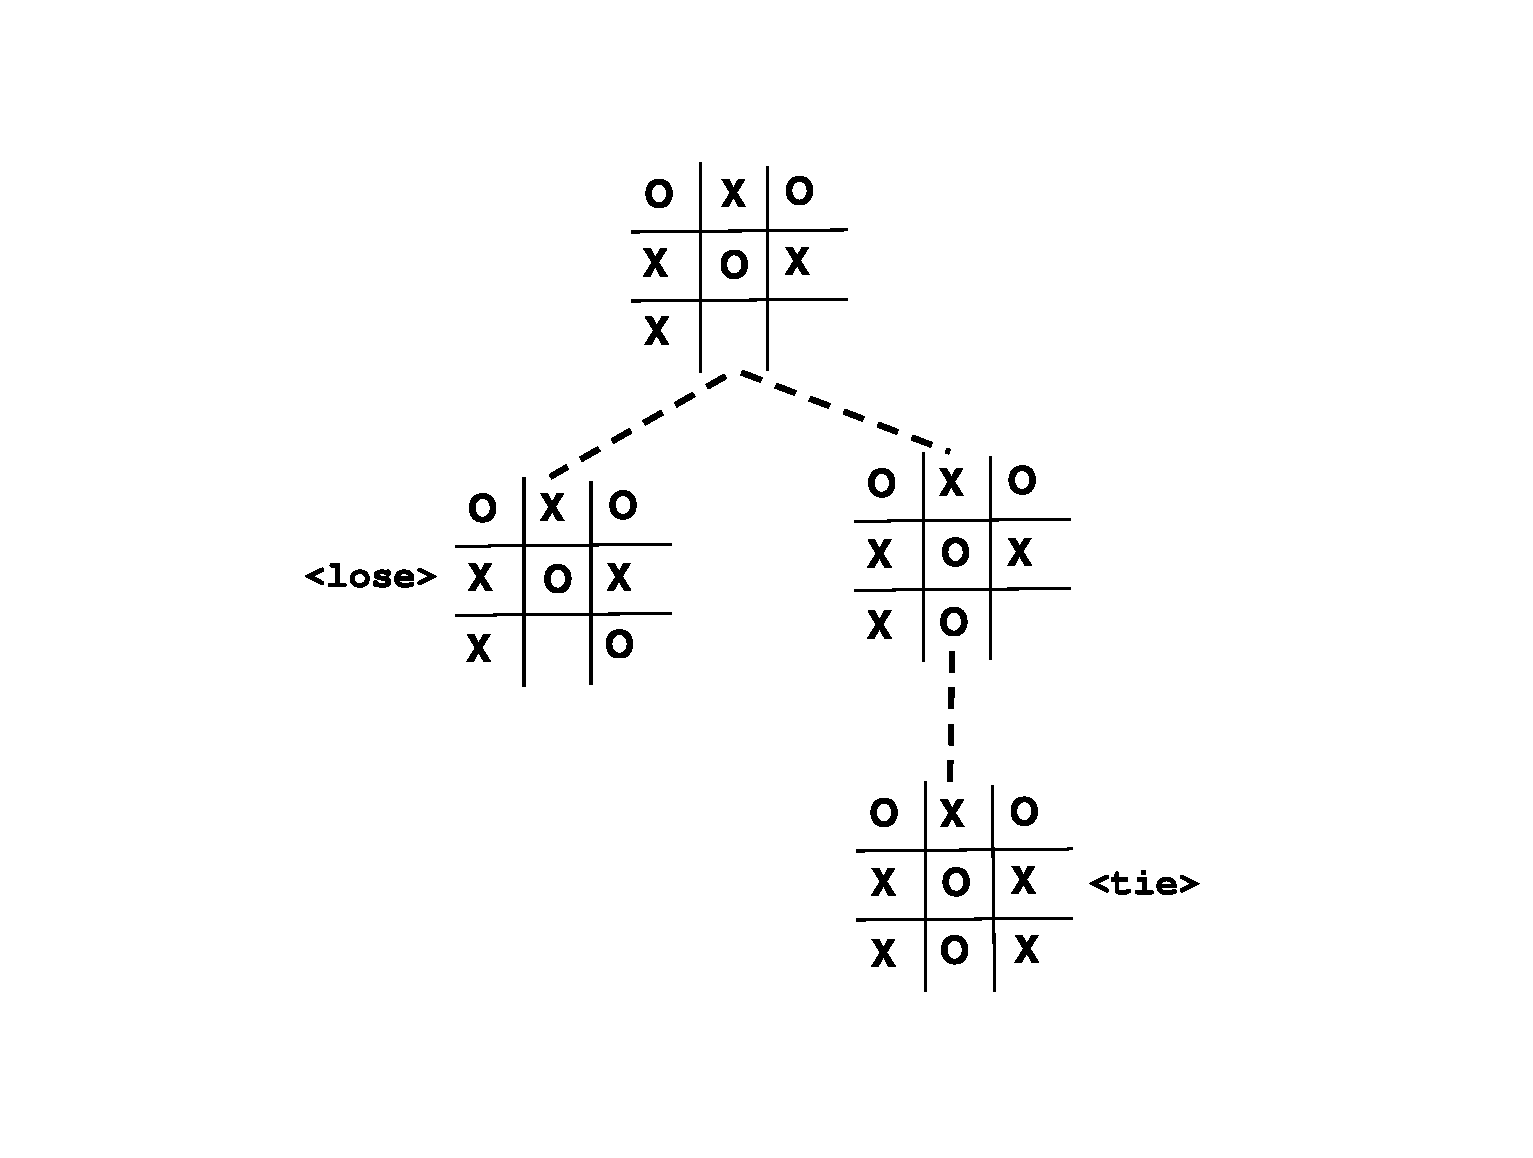
\includegraphics[width=6in]{endgame}
\caption{Game Tree for the Tic-Tac-Toe game starting at $P_0$.}
\label{fig:endgame}
\end{figure}

Game trees are usually pictured in this way with the starting pattern
(referred to as the ``root'' of the tree) at the top and lines connecting
the root to the \iffalse roots of the \fi game trees that start at each
possible next pattern.  The ``leaves'' at the bottom of the tree (trees
grow upside down in computer science) correspond to terminated games.  A
path from the root to a leaf describes a complete \emph{play} of the game.
(In English, ``game'' can be used in two senses: first we can say that
Chess is a game, and second we can play a game of Chess.  The first usage
refers to the data type of Chess game trees, and the second usage refers to
a ``play.'')

\subsection{Infinite Tic-Tac-Toe Games}

At any point in a Tic-Tac-Toe game, there are at most nine possible
next patterns, and no play can continue for more than nine moves.  But
we can expand Tic-Tac-Toe into a larger game by running a 5-game
tournament: play Tic-Tac-Toe five times and the tournament winner is
the player who wins the most individual games.  A 5-game tournament
can run for as many as 45 moves.

It's not much of generalization to have an \emph{$n$-game Tic-Tac-Toe
  tournament}.  But then comes a generalization that sounds simple but can
be mind-boggling: consolidate all these different size tournaments into a
single game we can call \emph{Tournament-Tic-Tac-Toe ($T^4$)}.  The first
player in a game of $T^4$ chooses any integer $n > 0$.  Then the players
play an $n$-game tournament.  Now we can no longer say how long a $T^4$
play can take.  In fact, there are $T^4$ plays that last as long as you
might like: if you want a game that has a play with, say, nine billion
moves, just have the first player choose $n$ equal to one billion.  This
should make it clear the game tree for $T^4$ is infinite.

But still, it's obvious that every possible $T^4$ play will stop.
That's because after the first player chooses a value for $n$, the
game can't continue for more than $9n$ moves.  So it's not possible to
keep playing forever even though the game tree is infinite.

This isn't very hard to understand, but there is an important
difference between any given $n$-game tournament and $T^4$: even
though every play of $T^4$ must come to an end, there is no longer any
initial bound on how many moves it might be before the game ends ---a
play might end after 9 moves, or $9(2001)$ moves, or $9(10^{10}+1)$
moves.  It just can't continue forever.

\begin{staffnotes}

While there is no bound on how long to play, at least after the
first move to an $n \times n$ board in meta-Tic-Tac-Toe, we know the game
will end with $n^2$ moves.

\end{staffnotes}

\iffalse
Now that we recognize $T^4$ as a \tg, we can go on to
a \emph{meta}-$T^4$ game, where the first player chooses a number,
$m>0$, of $T^4$ games to play, and then the second player gets the
first move in each of the individual $T^4$ games to be played.

Then, of course, there's meta-meta-$T^4$\dots.
\fi

\begin{staffnotes}
Every play of the meta-meta game must still end, but now even
after the first move, there is no bound on how long a game might
continue.
\end{staffnotes}

\subsection{Two Person Terminating Games}

Familiar games like Tic-Tac-Toe, Checkers, and Chess can be assigned
scores of 1, -1, or 0 corresponding to win, lose, or draw.  The game of Go
is often scored by counting the difference in the numbers of locations
controlled by the two players.  An $n$-game tournament of win, lose draw
games might be scored by adding up the scores of the individual games,
which would equal the number of games won by the first player minus the
number they lost.  \iffalse A negative score would mean the second player
won more games.\fi

The idea behind the definition of $\tg$'s as a recursive data type is that
making a move in a $\tg$ leads to the start of a subgame, as illustrated
by Tic-Tac-Toe and Tournament-Tic-Tac-Toe examples.  So given any set of
games, we can make a new game whose first move is to pick a game to play
from the set.  At the end of play there is a score.

So what defines a game?  For Tic-Tac-Toe, we used the patterns and the
rules of Tic-Tac-Toe to determine the next patterns.  But once we have
a complete game tree, we don't really need the pattern labels: the
root of a game tree itself can play the role of a ``board position''
with its possible ``next positions'' determined by the roots of its
subtrees.  So any game is defined by its game tree.  This leads to the
following very simple ---perhaps deceptively simple ---general
definition.

%\hyperdef{2p}{tg}{$\tg$}
\begin{definition}\label{tgdef}
  Let $S$ be a set of real numbers whose members will be called
  \emph{scores}. The \emph{game trees for $S$-scored two-person
    terminating games of perfect information} are defined recursively as
  follows:
\begin{itemize}

\item \textbf{Base case:}
\[
\ang{\textbf{leaf}, s} \in \tg,
\]
for all $s \in S$.

\item \textbf{Constructor case:}
If $\mathcal{G}$ is a nonempty set of
$\tg$'s, then $G$ is a $\tg$, where
\[
G \eqdef \ang{\textbf{tree},\mathcal{G}}.
\]
The game trees in $\mathcal{G}$ are called the possible \emph{next moves}
from $G$.
\end{itemize}

A \emph{play} of a $\tg$, $G$, is a (potentially infinite) sequence of
$\tg$'s starting with $G$ and such that if $G_1$ and $G_2$ are consecutive
$\tg$'s in the play, then $G_2$ is a possible next move of $G_1$.

If a $\tg$ has no infinite play, it is called a \emph{terminating} game.
\end{definition}

We already observed that even though the $T^4$ Tic-Tac-Toe tournament has
an infinite game tree, every play of $T^4$ must terminate.  We'll show
that this is true in general after we give a precise definition of
``play'':

\begin{theorem}
Every $\tg$ is terminating.
\end{theorem}

\begin{proof}
By structural induction on the definition of a $\tg$, $G$, with induction
hypothesis
\[
G \text{ is terminating}.
\]

\textbf{Base case}: If $G = \ang{\textbf{leaf}, s}$, then the only
possible play of $G$ is the length one sequence consisting of $G$ itself.
Hence $G$ terminates.

\textbf{Constructor case}: For $G = \ang{\textbf{tree},\mathcal{G}}$, we
must show that $G$ is terminating, given the structural induction
hypothesis that \emph{every} $G' \in \mathcal{G}$ is terminating.

Any play of $G$ is, by definition, a sequence starting with $G$ and
followed by a play starting with some $G_0 \in \mathcal{G}$.  But $G_0$ is
terminating, so the play starting at $G_0$ is finite, and hence so is the
play starting at $G$.

This completes the structural induction, proving that every \tg, $G$, is
terminating.
\end{proof}


\subsection{Game Strategies}

A key question about a game is what strategy will give a player the best
score.  A \emph{strategy} for a player in a game specifies which move the
player should make at any point in the game.

In Tic-Tac-Toe for example, most elementary school children figure out
strategies for both players that each guarantees a score of 0, that is, a
draw.  Of course the first player can win if his opponent plays
childishly, but not if the second player follows the proper strategy.  In
more complicated games like Checkers or Chess, it's not clear what
strategy, if any, is guaranteed to yield the best score.
But structural induction makes it easy to prove that in any $\tg$,
both players have strategies that guarantee the best possible score.

In particular, there are two players called the \term{max-player} and the
\term{min-player} who alternate making moves.  The score measures what the
max-player wins (it might be negative, indicating that the min-player came
out ahead).  The objective of the max-player is to have play end with as
high a score as possible, while the min-player aims to end with as low a
score as possible.

%%%%%%%%%%%%%%
Given which of the players moves first in a game, a strategy for the
max-player is said to \emph{ensure} the payoff, $s$, if play ends with a
score $ \ge k$, no matter what moves the min-player makes.  Likewise, a
strategy for the min-player is said to \emph{hold down} the score to $s$,
if play ends with a payoff of $\le s$, no matter what moves the max-player
makes.

A $\tg$ there are two values, a \term{max value} and a \term{min
  value}.   is said to have \emph{max value}, $s$, if the max-player has a
strategy that ensures payoff $k$, and the min-player has a strategy that
holds down the payoff to $k$, when the \emph{max-player moves first}.
Likewise, the $\tg$ has \emph{min value}, $k$, if the max-player has a
strategy that ensures $k$, and the min-player has a strategy that holds
down the payoff to $k$, when the \emph{min-player moves first}.

The \emph{Fundamental Theorem} for 2-person 50-point games of perfect
information is that is that every game has both a max value and a min
value.  (Note: the two values are usually different.)

What this means is that there's no point in playing a game: if the max
player gets the first move, the min-player should just pay the max-player
the max value of the game without bothering to play (a negative payment
means the max-player is paying the min-player).  Likewise, if the
min-player gets the first move, the min-player should just pay the
max-player the min value of the game.



PPART\label{finpg} Prove this Fundamental Theorem for 50-valued
$\tg$'s by structural induction.

SOLUTION

The proof is by structural induction on the definition of a
  $\tg$, $G$.  The induction hypothesis is that there is that
\begin{quote}
  $G$ has a max value and a min value.
\end{quote}

\textbf{Base case}: [$G$ is the terminated game with payoff $k$].  The only
possible play is $k$.  So the max value and the min value are both $k$.

\textbf{Constructor case}: [$G = (G_0,\dots, G_n)$].  By structural
induction we may assume that each of the games $G_i$ have both max values
and min values.

We first show that $G$ has max value, $k$, where $k$ is the largest min
value among the games $G_0,\dots,G_n$.

To prove the max value of $G$ is $k$, we must show how the max-player,
moving first in $G$, can ensure $k$, and how the min-player, moving second
in $G$, can hold down the payoff to $k$.

To ensure $k$, the max-player simply chooses $i$ as her first move where
game $G_i$ has this largest min value, $k$.  The min-player then has the
first move in $G_i$, so by definition of min value, the max-player has a
strategy in $G_i$ that ensures $k$, which she can now follow.  So this
first move, combined with the ensuring strategy in $G_i$, defines a
strategy for the max-player in $G$ that ensures $k$.

Likewise, there is a simple strategy for the min-player, moving second in
$G$, to hold down the payoff to $k$.  Namely, suppose the max-player's
first move is $i$.  Then $G_i$ has a min value of $m \leq k$, since $k$ is
the largest min value.  So by definition of min value, there is a strategy
in $G_i$ for the min-player to hold down the payoff to $m$, which he can
now follow, thereby holding down the payoff of play on $G$ to $m \leq k$.

The existence of these ensuring and holding down strategies for $G$
implies that the max value of $G$ is $k$.

Second, to show that $G$ has a min value, we can repeat the previous
argument with min and max exchanged.

Therefore, by structural induction, we can conclude that all $\tg$'s have
min and max values.

SOLUTION

PPART A meta-$\tg$ game has as possible first moves the choice of
\emph{any} $\tg$ to play.  Meta-$\tg$ games aren't any harder to
understand than $\tg$'s, but there is one notable difference, they
have an infinite number of possible first moves.  We could also define
meta-meta-$\tg$'s in which the first move was a choice of any
$\tg$ \emph{or} the meta-$\tg$ game to play.  In
meta-meta-$\tg$'s there are an infinite number of possible first
\emph{and} second moves.  And then there's $\text{meta}^3-\tg$ \dots.

\iffalse
The 2D-origin game in a Week 4 class problem is a game in which there are
an infinite number of possible first moves, an infinite number of possible
second moves, \dots.  \iffalse (with two values, ``win'' or ``lose''
instead of values from -50 to 50)\fi
\fi

To model such infinite games, we could have modified the recursive
definition of $\tg$'s to allow first moves that choose any one of an
infinite sequence
\[
G_0,G_1,\dots,G_n,G_{n+1}, \dots
\]
of $\tg$'s.  Now a $\tg$ can be a mind-bendingly infinite datum
instead of a finite one.

Do these infinite $\tg$'s still have max and min values?  In
particular, do you think it would be correct to use structural induction
as in part~\eqref{finpg} to prove a Fundamental Theorem for such infinite
$\tg$'s?  Offer an answer to this question, and briefly indicate why
you believe in it.

SOLUTION

It may not be obvious, but structural induction is a perfectly sound proof
technique even for infinite recursively defined data, and the proof of the
Fundamental Theorem for $\tg$'s applies without change to infinite ones.

SOLUTION

\begin{theorem}\label{fund}
  \textbf{Fundamental Theorem for Two-Person Games:} For every two-person
  terminating game of perfect information, has a max-value and a
  min-value.
\end{theorem}

\begin{proof}
The proof is by structural induction on the definition of a $\tg$, $G$.
The induction hypothesis is that there is a winning strategy for $G$.

\textbf{Base cases:}
\begin{enumerate}

\item $G=\ang{\textbf{leaf}, \textbf{win}}$.  Then the first player has the
 winning strategy: ``make the winning move.''

\item $G=\ang{\textbf{leaf}, \textbf{lose}}$.  Then the second player has a
 winning strategy: ``Let the first player make the losing move.''
\end{enumerate}

\textbf{Constructor case}: Suppose $G = \ang{\textbf{tree},\mathcal{G}}$.
By structural induction, we may assume that some player has a winning
strategy for each $G' \in \mathcal{G}$.  There are two cases to consider:
\begin{itemize}
\item some $G_0 \in \mathcal{G}$ has a winning strategy for its second
  player.  Then the first player in $G$ has a winning strategy: make the
  move to $G_0$ and then follow the second player's winning strategy in
  $G_0$.

\item every $G' \in \mathcal{G}$ has a winning strategy for its first
  player.  Then the second player in $G$ has a winning strategy: if the
  first player's move in $G$ is to $G_0 \in \mathcal{G}$, then follow the
  winning strategy for the first player in $G_0$.
\end{itemize}
So in any case, one of the players has a winning strategy for $G$, which
completes the proof of the constructor case.

It follows by structural induction that there is a winning strategy for
every $\tg$, $G$.
\end{proof}

Notice that although Theorem~\ref{fund} guarantees a winning strategy, its
proof gives no clue which player has it.  For the Subset Takeaway Game of
Problem~\ref{CP_subset_take_away} and most familiar $\tg$'s like Chess,
Go, \dots, no one knows which player has a winning
strategy.\footnote{Checkers used to be in this list, but there has been a
  recent announcement that each player has a strategy that forces a tie.
  (reference TBA)}

%% Games as a Recursive Data Type Problems %%%%%%%%%%%%%%%%%%%%%%%%%%%%%%%%%%%%
%\startclassproblems

\begin{problems}
%\classproblems
\homeworkproblems
%\pinput{PS_50_point_games}
\end{problems}
\fi

%% Induction in Computer Science %%%%%%%%%%%%%%%%%%%%%%%%%%%%%%%%%%%%%%%%%%%%%%
\section{Induction in Computer Science}

Induction is a powerful and widely applicable proof technique, which
is why we've devoted two entire chapters to it.  Strong induction and
its special case of ordinary induction are applicable to any kind of
thing with nonnegative integer sizes --which is a awful lot of things,
including all step-by-step computational processes.

Structural induction then goes beyond natural number counting by offering a
simple, natural approach to proving things about recursive computation
and recursive data types.  This makes it a technique every computer
scientist should embrace.

\begin{staffnotes}

In many cases a nonnegative integer size can be defined for a recursively
defined datum, such as the length of a string, or the number of operations
in an $\aexp$.  It is then possible to prove properties of data by ordinary
induction on their size.  But this approach often produces more cumbersome
proofs than structural induction.

In fact, structural induction is theoretically more powerful than ordinary
induction.  However, it's only more powerful when it comes to reasoning
about infinite data types ---like infinite trees, for example ---so this
greater power doesn't matter in practice.  What does matter is that for
recursively defined data types, structural induction is a simple and
natural approach.

\end{staffnotes}

\endinput


\begin{staffnotes}

\section{Tagged data}

Labelling a recursively defined data item with a tag that uniquely
determines the rule used to construct it is a standard approach to
avoiding ambiguous recursive definitions in programming.  This
amounts to working with data items that are already \term{parsed}, that
is, represented as \term{parse trees}.

For example, the parse tree for the arithmetic expression
\begin{equation}\label{ax}
-(a(x\cdot x)+ bx) + 1
\end{equation}
is shown in Figure~\ref{fig:parse}.

\begin{figure}
%\graphic{parsetree}
\inclludegraphics[width=5in]{parsetree}
\caption{Parse tree for $-(a(x\cdot x)+ bx) + 1$.}
\label{fig:parse}
\end{figure}

In a computer, such a tree would be represented by pairs or triples
that begin with a
\emph{tag} equal to the label of the top node of the parse tree.  
The general definition of parse trees for $\aexp$'s would be:

\newcommand{\paexp}{\text{Aexp-parse-tree}}

\begin{definition}\label{arithparse}
The set, $\paexp$, of \emph{parse trees for arithmetic expressions} 
over a set of
\emph{variables}, $V$, is defined recursively as follows:
\begin{itemize}
\item \textbf{Base cases:}
\begin{enumerate}
\item If $n \in \integers$, then $\ang{\texttt{int}, n} \in \paexp$.
\item If $v \in V$, then $\ang{\texttt{var}, v} \in \paexp$.
\end{enumerate}
\item \textbf{Constructor cases:} if $e,e' \in \paexp$, then
\begin{enumerate}
\item $\ang{\texttt{sum}, e, e'} \in \paexp$,
\item $\ang{\texttt{prod}, e, e'} \in \paexp$, and
\item $\ang{\texttt{minus}, e} \in \paexp$.
\end{enumerate}
\end{itemize}
\end{definition}

So the $\paexp$ corresponding to formula~\ref{ax} would be:
\begin{equation}\label{axtag}
\begin{array}{rll}
\left< \right. \texttt{sum}, 
         & \left< \right. \texttt{minus},\ \ \left< \right. \texttt{sum},
               & \ang{\texttt{prod},\ \ \ang{\texttt{var},\ a},
                                     \ang{\texttt{prod},\ \
                                            \ang{\texttt{var},\ x},\
                                            \ang{\texttt{var},\ x}}},\\
                               && \left. \left. \ang{\texttt{prod},\ \
                                       \ang{\texttt{var},\ b},\
                                       \ang{\texttt{var},\ x}}
                                   \right> \right>,\\
         & \left. \left. \ang{\texttt{int},\ 1} \right> \right>
\end{array}
\end{equation}
Now the expression~\ref{ax} is certainly a lot more humanly
intelligible than~\ref{axtag}, but~\ref{axtag} is in the
representation best suited and commonly used in compiling and
processing computer programs.

\end{staffnotes}


\begin{staffnotes}

\subsection{A String Theorem}

Here is a more complex proof, illustrating a combination of structural
induction and strengthening the hypothesis.

\begin{theorem}
  In a string of $0$s and $1$s, the number of occurrences of the pattern
  $01$ is less than or equal to the number of occurrences of $10$, plus
  one.
\end{theorem}

Let's try to prove this by structural induction.  First we must
define $P(s)$.  Let's write $\ms{num}(pat,s)$ as the number of
occurrences of the pattern string pat in s.  Now our inductive
hypothesis is
\[
P(s): \ms{num}(01,s) \leq \ms{num}(10,s) + 1. 
\]
If you try to prove this by structural induction, you will get
stuck.
Why? 
Consider what happens when you add $1$ at the end.  
This could increase the number of $01$s without increasing the number of
$10$s. 

So, to prove by structural induction on strings, let's strengthen the
hypothesis by adding another clause.  If a string ends in $0$ then
the number of $01$s is less than or equal to the number of $10$s.
That solves the problem by weakening what we have to show when the
string ends in $1$.  But maybe it causes another problem somewhere
else.  Let's give it a try:

Redefine $P(s) \eqdef$
\begin{eqnarray*}
\ms{num}(01,s) & \leq & \ms{num}(10,s) + 1, \text{ and}\\
\lefteqn{\text{If $s$ ends in $0$ then}}\\
\ms{num}(01,s) & \leq  &\ms{num}(10,s).
\end{eqnarray*} 
 
This means that, for each inductive step have two things to show.
\iffalse

\structuredproof{

  Prove: $\forall s \in S \; (P(s))$ \\
  1. (Base) $P(\emptystring)$ 
  \reason{No patterns of either kind.} \\
  2. (Inductive step) $\forall s \in S \; (P(s) \implies P(s 0))$ \\
  1. Fix $s$. \\
  2. Assume $P(s)$. \\
  3. $P(s 0)$ \\
  1. $\ms{num}(01,s0) \leq \ms{num}(10,s0) + 1$. 
  \reason{???} \\
  2. If $s 0$ ends in $0$ then $\ms{num}(01,s0) \leq
  \ms{num}(10,s0)$. \noreason \\
  \reason{???} \\
  3. QED
  \reason{Conjunction} \\
  4. QED 
  \reason{Implication, UG} \\
  3. (Inductive step) $\forall s \in S \; (P(s) \implies P(s 1))$ \\
  1. Fix $s$. \\
  2. Assume $P(s)$. \\
  3. $P(s 1)$ \\
  1. $\ms{num}(01,s1) \leq \ms{num}(10,s1) + 1$. 
  \reason{???} \\
  2. If $s 1$ ends in $0$ then $\ms{num}(01,s1) \leq
  \ms{num}(10,s1)$.\noreason \\
  \reason{???} \\
  3. QED
  \reason{Conjunction} \\
  4. QED 
  \reason{Implication, UG} \\
  4. QED
  \reason{Structural induction on strings.}\\
}\fi

\textcolor{blue}{Structured proof display commented out here}

First let's consider $s1$. This is the case that looks dangerous,
because it might increase the number of $01$s.  We have to prove two
statements.  The second is easy, because the new string doesn't end in
$0$.  We say it's ``vacuously true''.

The first statement now takes some work. 
We might be adding to the number of $01$s.  
However, if we do, the previous string must have ended with $0$. 
Then the inductive hypothesis says that the previous string had to
satisfy the stronger inequality in the second statement. 
Adding one to the LHS of the stronger inequality yields the weaker
inequality we want.

The following proof fragment considers cases based on whether $s$ ends
in $0$ or not.  If not, it might end in $1$, or might be empty (don't
forget this possibility).

\textcolor{blue}{Structured proof display commented out here}
\iffalse

\begin{proof}
  3. $P(s 1)$ \\
  1. $\ms{num}(01,s1) \leq \ms{num}(10,s1) + 1$. \\
  1. If $s$ ends in $0$ then $\ms{num}(01,s1) \leq\ms{num}(10,s1) + 1$. \\
  1. Assume $s$ ends in $0$. \\
  2. $\ms{num}(01,s) \leq \ms{num}(10,s)$ 
  Inductive hypothesis (3.2), part 2. \\
  3. $\ms{num}(01,s1) = \ms{num}(01,s) + 1$ 
  Adding one more $01$. \\
  4. $\ms{num}(10,s1) = \ms{num}(10,s)$ \\
  5. $\ms{num}(01,s1) \leq\ms{num}(10,s1) + 1$. 
  Algebra (combining 3.3.1.1.2, ...3, and ...4) \\
  QED 
  Implication \\
  2. If $s$ ends in $1$ then $\ms{num}(01,s1)\leq\ms{num}(10,s1) + 1$. \\
  Inductive hypothesis, part 1; no new $01$s. \\
  3. If $s = \emptystring$ then $\ms{num}(01,s1) \leq\ms{num}(10,s1)+ 1$. \\
  $s1$ is just $1$, which has no $01$s. \\
  4. QED 
  Cases \\
  2. If $s 1$ ends in $0$ then $\ms{num}(01,s1) \leq \ms{num}(10,s1)$. \\
  Vacuously true, because $s1$ doesn't end in $0$. \\
  3. QED
  Conjunction \\
\end{proof}
\fi

Of course, you could also expand the step for $s$ ending in $1$ into a
careful series of inequalities.

Now consider $s0$.  We hope that what we did to make the $s1$ case
work doesn't mess up the $s0$ case.  But we have to check.

The first statement is easy.  It follows from the first statement of
the inductive hypothesis for $s$, because we are not increasing the
number of $01$s.  But now the second statement takes more work.  The
difficulty is that the new string ends in $0$, which means that we
have to show the stronger inequality in the second statement.  But to
do this, we might only have the weaker inequality for the previous
string.  The argument again depends on what the previous string $s$
ended with.  So again, we consider cases, based on whether $s$ ends in
$0$ or $1$, or is empty.  If $s$ ends in $0$ we rely on the second
statement of the inductive hypothesis for $s$ (with the stronger
inequality), whereas if $s$ ends in $1$ we rely on the first statement
(with the weaker inequality).  In this case, we have to ``turn the
weaker inequality into the stronger inequality''.

\iffalse
\structuredproof[38ex]{
  3. $P(s 0)$ \\
  1. $\ms{num}(01,s0) \leq \ms{num}(10,s0) + 1$.
  \reason{Induct. hypothesis, part 1; no new $01$s.} \\
  2. If $s 0$ ends in $0$ then $\ms{num}(01,s0) \leq\ms{num}(10,s0)$. \\
  1. $\ms{num}(01,s0) \leq \ms{num}(10,s0)$. \\
  1. If $s$ ends in $0$ then $\ms{num}(01,s0)
  \leq\ms{num}(10,s0)$. \noreason \\
  \reason{Induct. hypothesis, part 2; no new $01$s} \\
  2. If $s$ ends in $1$ then $\ms{num}(01,s0)
  \leq\ms{num}(10,s0)$. \noreason \\ 
  1. Assume $s$ ends in $1$. \\
  2. $\ms{num}(01,s) \leq \ms{num}(10,s) + 1$. 
  \reason{Inductive hypothesis, part 1} \\
  3. $\ms{num}(01,s0) = \ms{num}(01,s)$ \\
  4. $\ms{num}(10,s0) = \ms{num}(10,s) + 1$ 
  \reason{Exactly one new occurrence of $10$.} \\
  5. $\ms{num}(01,s0) \leq \ms{num}(10,s0)$ 
  \reason{Algebra} \\
  6. QED
  \reason{Implication} \\
  3. If $s = \emptystring$ then $\ms{num}(01,s0) \leq
  \ms{num}(10,s0)$. \noreason \\ 
  
\reason{$s0$ is just $1$, which has no $01$s or $10$s.} \\
  4. QED 
  \reason{Cases} \\
  2. QED
  \reason{Propositional reasoning (truth table)} \\
  3. QED 
  \reason{Conjunction}\\
}
\fi

\textcolor{blue}{Structured proof display commented out here}

If you actually write out all these cases in the proof, you will
notice that some facts are stated repeatedly, e.g., that when you add
a $0$ to the end of a string you are not increasing the number of
$01$s.  To avoid having to state these facts several times, you can
move them earlier in the proof.

\end{staffnotes}
